\chapter{Service-oriented computing}
\label{chap:service-oriented computing}
\emph{Service-oriented computing} represents a distributed computing platform. [1] It has its own paradigm, logic, architecture and patterns. It is built on the distributed computing platforms and extends it by new considerations about governance, design layers and technologies suitable for its implementation.
\emph{Service orientation} is a design paradigm, it divides the system into logic units which are separately shaped and can be utilized according to strategic goals and benefits of a requested result.

\section{Service-oriented architecture}
\emph{Service-oriented architecture (SOA)} is a set of best practices for an organization leading to agile architectural model of the system to meet business needs. Result of applied practices is an architecture which corresponds to dynamic market changes. The SOA best practices are describing the human behaviour, there is no list of constraints which have to be followed to obtain a service-oriented architecture. The best practices are designed to resolve specific situations which the organization can meet and depending on them could be selected just a subset of appropriate practices which are necessary to apply.

The architecture is layered. Layers can be multiple and can differ according to needs of designed system. One of the expamles of horizontal layers is designed in picture \ref{fig:soa-architecture}.

\begin{figure}[htp] \centering{
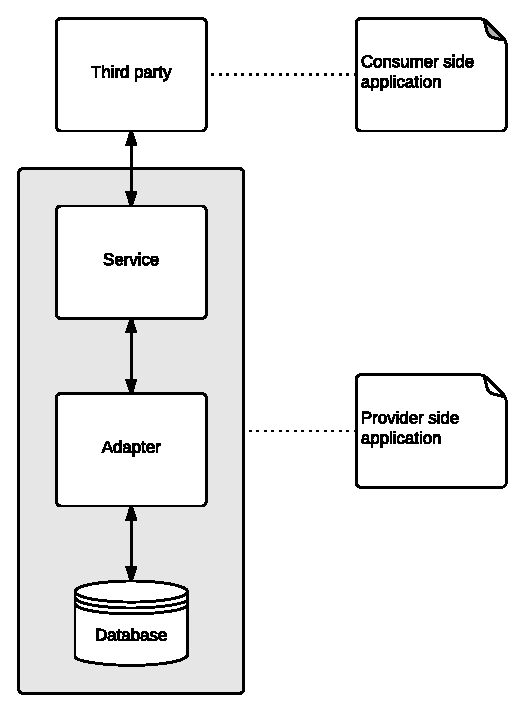
\includegraphics[width=8cm]{img/soa-architecture.pdf}}
\caption{Example of service-oriented architecture model}
\label{fig:soa-architecture}
\end{figure}  

One of the main advantages of a service-oriented architectural style is its ability to efficiently deal with changes. "SOA is based on a decomposition of enterprise IT assets and separation of "stable" IT artifacts (services) from "changeable" artifacts (business processes), orchestrating services into IT solutions (processes)." \cite{website:versioning-in-soa}. %(http://msdn.microsoft.com/en-us/library/bb491124.aspx) 
Above mentioned services are essential part of SOA. Relationship between them and a business process constituted by services is visualized in the picture \ref{fig:business-process-services}.

\begin{figure}[htp] \centering{
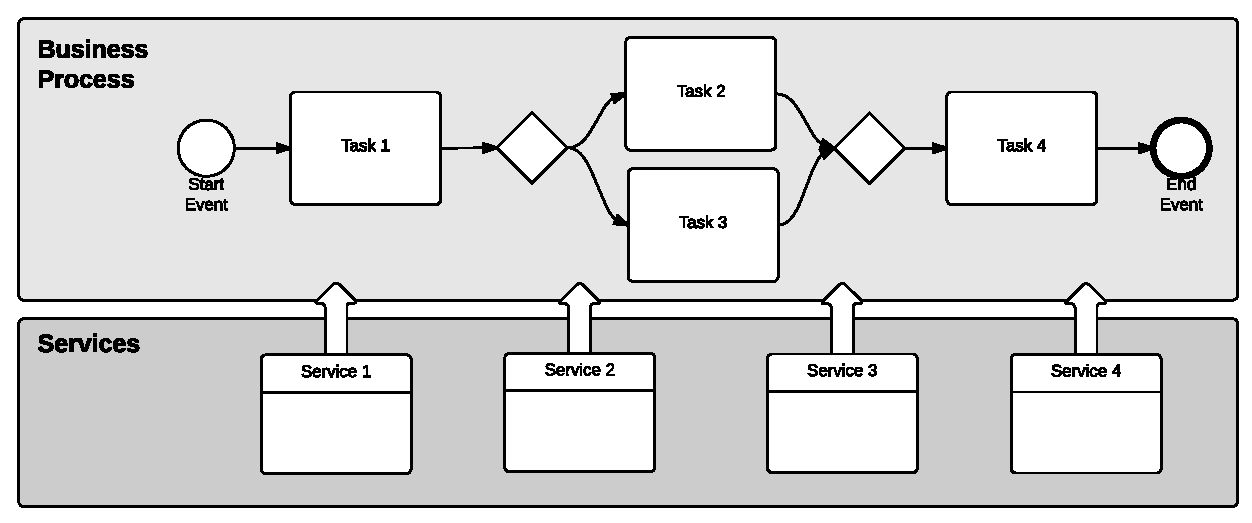
\includegraphics[width=12cm]{img/business-process-services.pdf}}
\caption{Business process is a composition of services}
\label{fig:business-process-services}
\end{figure} 

The speed of changes in the bussines department is too fast to be passed directly into development and maintance of the monolitic systems. Funcionality of these systems is designed on measure of customer and often can't deal easily with changes, it can arrive in interference in design of whole architecture. SOA offers better flexibility when business requirements change, changes are refleted into modification of an existing business process by changing involved services, or if it's needed a new process is created using existing services or a new service can be created. There are more approaches how to deal with the changes and one of them is versioning which is described in chapter \ref{chap:versioning} and \ref{chap:versionaccess} in detail.





\section{Services}
\label{sec:services}
Services are the logic units form which is composed the \gls{service-oriented-design}. Every service is standalone object or component. Every service has its own functional context and related capabilities. Each service is deployerd independetly on another one and on the system which use it. It allows a parallel development, one service can be a part of many products of the corporation.
The essence of Service in the SOA context is the business abstraction - that is a representation of funcionality and/or data presented in business context \cite{agile-architecture}.

\subsection{Levels of a service} 
\label{subsec:levels-of-serivce}

There are three levels of how we can interpret the expression \emph{'Service'} in SOA context \cite{agile-architecture}:
\begin{enumerate}
  \item \textbf{Service implementation} \hfill \\
Service implementation is the code performing the logic.
  \item \textbf{Service interface} \hfill \\ 
This level is an entry point to the sevice implmentation, it provides underlying logic to consumers but encapsulating it in a way that consumers can see the implementation. 
  \item \textbf{Abstracted service} \hfill \\
Abstracted service or business service represents a business capability or data. This services can be composed to describe a business process. This is a core abstraction of SOA.
\end{enumerate}

There is a many-to-many relationship between these three levels. Business service can represents muliple interfaces and in the same time one interface can be supported by multiple implementation.

/TODO image

\subsection{Service categories and types} \cite{website:ontology-taxonomy}

There are two main types of services. The first type is composed by infrastructural services which provide the facilities and aren't a part of application. To the second type belongs services which are the part of the application and provide main logic.

/TODO decribe services

\begin{description}
  \item[Bus services] can be further divided into 
  \begin{enumerate}
    \item Communication services 
    \item Utility services
  \end{enumerate}
  \item[Application services] consist of   
  \begin{enumerate}
    \item Entity services
    \item Capability services
    \item Activity services
    \item Process services
  \end{enumerate}
\end{description}

/TODO image

\section{Services granularity}
\label{sec:granularity}
During the analytical part of the service design it can be defined the service granularity. The service granularity describes functional scope of the serivce. When the granularity is fine, it means the service contains little logic. On the other hand there are coarse-grained serices which have complex logic but at the expense of flexibility.
Defining the granularity can help to determine the characteristics of the serivce - its performance or size of message. \cite{soa-contract}

\section{Approaches of implementation of web services}
Web services are one group of services, these are intended to work on a network such as Internet.

\subsection{Evolution of approches}
\subsubsection{WSDL RPC SOAP} 
/TODO form agile arcitecture revolution
 
\subsection{REST}
/TODO WADL

Representational State Transfer, REST is an architectural style for building ditributed hypermedia applications.
Thanks to REST disappeared many issues related to web services, but it comes with some new. This thesis deals with REST style and RESTfull services. \ref{chap:rest}

%%\subsubsection*{\textbf{Guacamole} \hfill \emph{http://guac-dev.org/}}
%%\label{subsec:guacamole}
%% \ref{}.
%%    \item \textbf{[název předmětu 1]} \hfill \\
%%    odkaz na stránku předmětu, obsahující pouze název a informace o spolufinancování \gls{eu}
    
%%\begin{table}
%%  \caption{Základní typy entit v Drupalu}
  %%\label{tab:typy-entit}
  %%\begin{tabular}{ | p{3cm} | l | c | c | }
   %% \hline 
    %%Typ entity & Strojový název & Dostupnost polí & Rozšiřitelnost \\ \hline 
    %%Komentář & comment & \checkmark & \checkmark \\ \hline 
    %%Soubor & file &  & \\ \hline 
    %%Slovník & vocabulary &  & \\ \hline 
    %%Uzel & node & \checkmark & \checkmark \\ \hline 
    %%Uživatel & user & \checkmark & \checkmark \\ \hline 
    %%Záznam slovníku & term & \checkmark & \checkmark \\ \hline             
  %%\end{tabular}
%%\end{table}
%% \emph \emph \texttt.

